%%% CSE 4316 ADS - WORKED EXAMPLE (Computer Vision / ML). Follows ISO/IEC/IEEE 42010:2022 + IEEE 1016-2009.
\documentclass[11pt,letterpaper]{article}
\usepackage[margin=1.0in]{geometry}
\usepackage[T1]{fontenc}\usepackage[bitstream-charter]{mathdesign}\usepackage[latin1]{inputenc}
\usepackage{amsmath}\usepackage{xcolor}\usepackage{cite}\usepackage{hyphenat}
\usepackage{graphicx}\usepackage{float}\usepackage{subfigure}\usepackage{sectsty}
\usepackage[compact]{titlesec}\usepackage[tablegrid]{vhistory}\usepackage{pbox}\usepackage{longtable}
\usepackage{tikz}\usetikzlibrary{positioning,arrows.meta,fit,backgrounds}
\allsectionsfont{\color{accentcolor}\scshape\selectfont}
\definecolor{accentcolor}{rgb}{0.0,0.0,0.5}
\tikzset{
  mod/.style={draw, rounded corners, fill=white, minimum height=8mm, minimum width=27mm, font=\footnotesize, align=center, inner sep=2pt},
  ext/.style={draw, dashed, rounded corners, fill=black!4, minimum height=8mm, minimum width=24mm, font=\footnotesize\itshape, align=center, inner sep=2pt},
  band/.style={draw=accentcolor!45, rounded corners, inner sep=3.5mm},
  llbl/.style={font=\small\bfseries, text=accentcolor, align=left},
  flow/.style={-{Latex[length=2mm]}, thick, draw=accentcolor!80},
  fl/.style={font=\scriptsize, fill=white, inner sep=1pt},
}
\newcommand{\teamname}{Team Perceptron}
\newcommand{\productname}{DigitDesk Handwritten Form Digitization Service}
\newcommand{\coursename}{CSE 4316: Senior Design I}
\newcommand{\semester}{Fall 2026}
\newcommand{\docname}{Architectural Design Specification}
\newcommand{\department}{Department of Computer Science \& Engineering}
\newcommand{\university}{The University of Texas at Arlington}
\newcommand{\authors}{Alan Turing \\ Grace Hopper \\ John Von Neumann \\ Ada Lovelace \\ Charles Babbage}
\usepackage{fancyhdr}\pagestyle{fancy}\usepackage{lastpage}
\lhead{}\chead{}\rhead{}\lfoot{\footnotesize \teamname \ - \semester}\cfoot{}
\rfoot{\footnotesize page \thepage\ of \pageref{LastPage}}
\renewcommand{\headrulewidth}{0.0pt}\renewcommand{\footrulewidth}{0.4pt}
\usepackage[runin]{abstract}\abslabeldelim{\quad}\setlength{\abstitleskip}{-10pt}
\renewcommand{\abstractname}{}\renewcommand{\abstracttextfont}{\color{accentcolor} \small \slshape}

\begin{document}
{\centering \huge \color{accentcolor} \sc \textbf{\department \\ \university} \par}
\vspace{1 in}
{\centering \huge \color{accentcolor} \sc \textbf{\docname \\ \coursename \\ \semester} \par}
\vspace{0.5 in}
\begin{figure}[h!]\centering
\includegraphics[width=0.60\textwidth]{images/test_image}\end{figure}
\vspace{0.5 in}
{\centering \huge \color{accentcolor} \sc \textbf{\teamname \\ \productname} \par}
\vspace{0.5 in}{\centering \large \sc \textbf{\authors} \par}
\newpage
\begin{versionhistory}
  \vhEntry{0.1}{11.02.2026}{JVN}{document creation}
  \vhEntry{1.0}{11.18.2026}{AT|GH|CB}{official release}
\end{versionhistory}
\newpage\setcounter{tocdepth}{2}\tableofcontents\newpage

\section{Introduction}
Architecture of \productname\ as an ISO/IEC/IEEE 42010:2022 \cite{ISO42010}
architecture description using IEEE 1016-2009 \cite{IEEE1016} viewpoints. Refines
the SRS. Scope: the on-prem service, its REST API, and the review UI.

\section{Stakeholders \& Architectural Concerns}
\begin{table}[H]\begin{center}\begin{tabular}{ | p{3.5cm} | p{9.5cm} |}\hline
\textbf{Stakeholder} & \textbf{Primary concerns} \\ \hline
Sponsor (records office) & accuracy, auditability, on-prem data handling, cost \\ \hline
Clerks (reviewers) & fast, clear review workflow \\ \hline
IT administrator & deployability, monitoring, security \\ \hline
Development team & feasibility, modular/replaceable model, testability \\ \hline
\end{tabular}\end{center}\end{table}

\section{Architecture Viewpoints}
Context (Section 4), Composition/Data Flow (Section 5), Logical/Functional
(Sections 6--8), Deployment (Section 8). Style: a containerized pipeline of
services communicating over an internal message queue and HTTP, deployed on-prem.
Interfaces use \texttt{\#NN}; subsystems named \texttt{[Layer].[Name]}.

\section{System Overview \& Context View}
\begin{figure}[h!]\centering\resizebox{0.95\textwidth}{!}{%
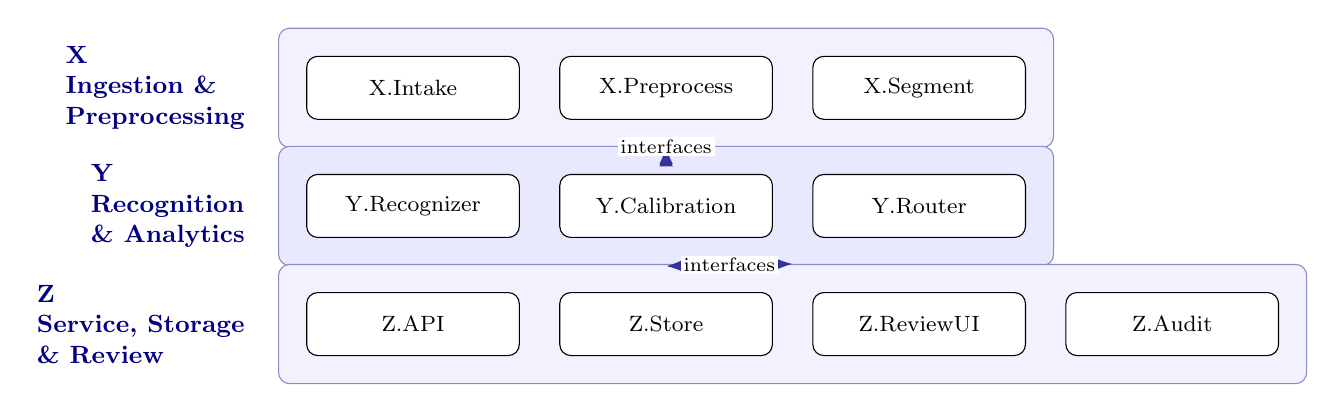
\begin{tikzpicture}[node distance=5mm]
\node[mod] (xin) {X.Intake};
\node[mod, right=of xin] (xpre) {X.Preprocess};
\node[mod, right=of xpre] (xseg) {X.Segment};
\node[mod, below=15mm of xin.west, anchor=west] (yrec) {Y.Recognizer};
\node[mod, right=of yrec] (ycal) {Y.Calibration};
\node[mod, right=of ycal] (yrou) {Y.Router};
\node[mod, below=15mm of yrec.west, anchor=west] (zapi) {Z.API};
\node[mod, right=of zapi] (zsto) {Z.Store};
\node[mod, right=of zsto] (zrev) {Z.ReviewUI};
\node[mod, right=of zrev] (zaud) {Z.Audit};
\begin{scope}[on background layer]
\node[band, fill=blue!5, fit=(xin)(xseg)] (bx) {};
\node[band, fill=blue!9, fit=(yrec)(yrou)] (by) {};
\node[band, fill=blue!5, fit=(zapi)(zaud)] (bz) {};
\end{scope}
\node[llbl, left=3mm of bx] {X\\Ingestion \&\\Preprocessing};
\node[llbl, left=3mm of by] {Y\\Recognition\\\& Analytics};
\node[llbl, left=3mm of bz] {Z\\Service, Storage\\\& Review};
\draw[{Latex}-{Latex}, thick, draw=accentcolor!80] (bx.south) -- (by.north) node[fl,midway]{interfaces};
\draw[{Latex}-{Latex}, thick, draw=accentcolor!80] (by.south) -- (bz.north) node[fl,midway]{interfaces};
\end{tikzpicture}}
\caption{Three-layer pipeline: ingestion, recognition, service}\end{figure}
External actors: the scan workflow (submits images to the API), the clerk (review
UI), and the downstream records database (consumes verified export). X ingests and
prepares images; Y recognizes and routes; Z serves, stores, reviews, and audits.

\section{Subsystem Definitions \& Data Flow}
\begin{figure}[h!]\centering\resizebox{\textwidth}{!}{%
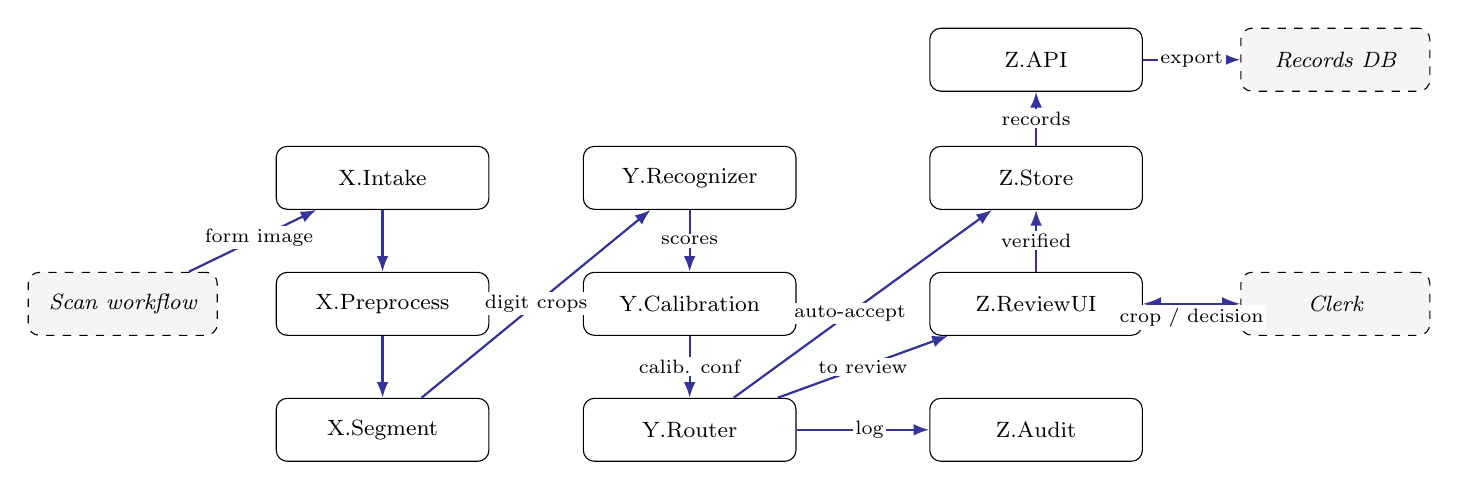
\begin{tikzpicture}
\node[ext] (scan) at (0,0) {Scan workflow};
\node[mod] (xin)  at (3.3,1.6) {X.Intake};
\node[mod] (xpre) at (3.3,0)   {X.Preprocess};
\node[mod] (xseg) at (3.3,-1.6){X.Segment};
\node[mod] (yrec) at (7.2,1.6) {Y.Recognizer};
\node[mod] (ycal) at (7.2,0)   {Y.Calibration};
\node[mod] (yrou) at (7.2,-1.6){Y.Router};
\node[mod] (zapi) at (11.6,3.1){Z.API};
\node[mod] (zsto) at (11.6,1.6){Z.Store};
\node[mod] (zrev) at (11.6,0)  {Z.ReviewUI};
\node[mod] (zaud) at (11.6,-1.6){Z.Audit};
\node[ext] (clerk) at (15.4,0) {Clerk};
\node[ext] (recdb) at (15.4,3.1){Records DB};
\draw[flow] (scan) -- (xin) node[fl,pos=0.55]{form image};
\draw[flow] (xin) -- (xpre);
\draw[flow] (xpre) -- (xseg);
\draw[flow] (xseg) -- (yrec) node[fl,pos=0.5]{digit crops};
\draw[flow] (yrec) -- (ycal) node[fl,pos=0.5]{scores};
\draw[flow] (ycal) -- (yrou) node[fl,pos=0.5]{calib. conf};
\draw[flow] (yrou) -- (zsto) node[fl,pos=0.45]{auto-accept};
\draw[flow] (yrou) -- (zrev) node[fl,pos=0.5]{to review};
\draw[flow] (yrou) -- (zaud) node[fl,pos=0.55]{log};
\draw[{Latex}-{Latex}, thick, draw=accentcolor!80] (zrev) -- (clerk) node[fl,pos=0.5,below]{crop / decision};
\draw[flow] (zrev) -- (zsto) node[fl,pos=0.5]{verified};
\draw[flow] (zsto) -- (zapi) node[fl,pos=0.5]{records};
\draw[flow] (zapi) -- (recdb) node[fl,pos=0.5]{export};
\end{tikzpicture}}
\caption{Image $\rightarrow$ preprocess $\rightarrow$ segment $\rightarrow$ recognize $\rightarrow$ route $\rightarrow$ store/review}\end{figure}

\section{X Layer Subsystems --- Ingestion \& Preprocessing}
\subsection{X.Intake}
\textbf{Responsibilities:} accept uploads (EI-01), assign a job id, enqueue work.
\begin{table}[H]\begin{center}\begin{tabular}{ | p{1cm} | p{6cm} | p{2.6cm} | p{2.6cm} |}\hline
ID & Description & Inputs & Outputs \\ \hline
\#01 & Ingestion API & form image & job id, queued image \\ \hline
\end{tabular}\end{center}\end{table}
\subsection{X.Preprocess}
\textbf{Responsibilities:} deskew, denoise, binarize to a normalized page.
\subsection{X.Segment}
\textbf{Responsibilities:} locate numeric fields on the known template and emit
per-field digit crops (FR-01). \textbf{Rationale:} template-anchored segmentation is
robust and simple for a fixed form (AD-01).

\section{Y Layer Subsystems --- Recognition \& Analytics}
\subsection{Y.Recognizer}
\textbf{Responsibilities:} classify digit crops and output values with raw scores
(FR-02). Model is a replaceable artifact (QA-01).
\begin{table}[H]\begin{center}\begin{tabular}{ | p{1cm} | p{6cm} | p{2.6cm} | p{2.6cm} |}\hline
ID & Description & Inputs & Outputs \\ \hline
\#02 & Recognition & digit crops & values, raw scores \\ \hline
\end{tabular}\end{center}\end{table}
\subsection{Y.Calibration}
\textbf{Responsibilities:} convert raw scores to calibrated confidences (temperature
scaling), so routing thresholds are meaningful (supports PE-02, FR-03).
\subsection{Y.Router}
\textbf{Responsibilities:} apply the acceptance threshold (FR-03) --- auto-accept or
enqueue for review.

\section{Z Layer Subsystems --- Service, Storage \& Review}
\subsection{Z.API}
\textbf{Responsibilities:} REST surface, authentication (SE-02), job status, export
(FR-05). \textbf{Deployment:} containers orchestrated on the on-prem host.
\subsection{Z.Store}
\textbf{Responsibilities:} persist images, results, and versions (MS-01); on-prem
only (SE-01).
\subsection{Z.ReviewUI}
\textbf{Responsibilities:} present queued fields for confirm/correct (FR-04).
\subsection{Z.Audit}
\textbf{Responsibilities:} append-only log of every field decision (FR-05, SE-02).

\section{Architecture Decisions \& Rationale}
\subsection{AD-01: Template-anchored segmentation}
\textbf{Context:} fixed form layout (FR-01). \textbf{Decision:} anchor fields to the
template rather than learn detection. \textbf{Alternatives:} learned detector (more
data, more risk). \textbf{Consequences:} simple and robust now, less general (see
FI-01). \textbf{Affects:} FR-01.
\subsection{AD-02: Calibrated confidence for routing}
\textbf{Context:} FR-03/PE-02 depend on trustworthy confidence. \textbf{Decision:}
add a calibration stage. \textbf{Alternatives:} raw softmax (poorly calibrated).
\textbf{Consequences:} extra stage, but auto-accept error stays bounded. \textbf{Affects:} FR-02, FR-03, PE-02.

\section{Requirements Traceability}
\begin{table}[H]\begin{center}\begin{tabular}{ | p{2cm} | p{5.5cm} | p{5cm} |}\hline
\textbf{Req ID} & \textbf{Requirement (abbrev.)} & \textbf{Realizing subsystem(s)} \\ \hline
FR-01 & Field segmentation & X.Segment \\ \hline
FR-02 & Recognition + confidence & Y.Recognizer, Y.Calibration \\ \hline
FR-03 & Confidence routing & Y.Router \\ \hline
FR-04 & Human review & Z.ReviewUI \\ \hline
FR-05 & Export \& audit & Z.API, Z.Audit \\ \hline
SE-01 & On-prem data & Z.Store \\ \hline
\end{tabular}\end{center}\end{table}

\bibliographystyle{reference/IEEEtran_custom}
\bibliography{reference/refs}{}
\end{document}
